\documentclass[twoside]{article}
\usepackage[layout=letterpaper,margin=1in]{geometry}

\usepackage{bold-extra} % for bf sc

\usepackage{amsmath} % For \text, \underbrace
\usepackage{amssymb} % For \checkmark
\usepackage{color}
\usepackage{comment}
\usepackage{fancyhdr}
\usepackage{graphicx}
\usepackage{listings}
\usepackage{longtable}
\usepackage{marginnote}
\usepackage{multirow}
\usepackage{nth}
\usepackage{subcaption}
\usepackage{soul} % provides \hl{}
\newcommand{\hlc}[2][yellow]{{\sethlcolor{#1}\hl{#2}}}
\usepackage{tabu}
\usepackage{tabularx}
\usepackage[normalem]{ulem} % provides \uline{}
\usepackage{varwidth}
\usepackage{xfrac}   % For \sfrac
\usepackage{xspace}

\usepackage[all=normal,lists]{savetrees}

\usepackage{rotating}
\usepackage[endianness=big]{bytefield}
%\bytefieldsetup{boxformatting={\centering\footnotesize}}

\usepackage{
  tikz,
  tikz-timing,
}
\usetikzlibrary{positioning}

\usepackage[colorlinks=true,bookmarksopen=true,bookmarksopenlevel=2]{hyperref}

\newcommand{\colorbitbox}[3]{%
\rlap{\bitbox{#2}{\color{#1}\rule{\width}{\height}}}%
\bitbox{#2}{#3}}

\newcommand{\prefix}[4]{%
\colorbitbox{lightgray}{1}{#1}
\colorbitbox{lightgray}{1}{#2}
\colorbitbox{lightgray}{1}{#3}
\colorbitbox{lightgray}{1}{#4}
}

\newcommand{\fuid}[4]{%
\bitbox{1}{\tt #1}
\bitbox{1}{\tt #2}
\bitbox{1}{\tt #3}
\bitbox{1}{\tt #4}
}

\newcommand{\fuaddr}[8]{
\begin{bytefield}{8}
  \bitheader{0-7} \\
  \prefix{#1}{#2}{#3}{#4}
  \fuid{#5}{#6}{#7}{#8}
\end{bytefield}
}

\definecolor{lightblue}{RGB}{0,204,255}
\definecolor{lightcyan}{rgb}{0.84,1,1}
\definecolor{lightgreen}{rgb}{0.64,1,0.71}
\definecolor{lightergreen}{rgb}{0.84,1,0.87}
\definecolor{lightred}{rgb}{1,0.7,0.71}

\newcommand{\bus}{MBus\xspace}
\newcommand{\mbuscopy}{MBus~\textcopyright~$2012-2015$~The Regents of the University of Michigan}

%%%%%%%%%%%%%%%%%%%%%%%%%%%%%%%%%%%%%%%%%%%%%%%%%%%%%%%%%%%%%%%%%%%%%%%%%%%%%%%%
\begin{document}

\pagestyle{fancyplain}

\fancyfoot[LO,RE]{\footnotesize \ifnum\thepage=1 ~\else \mbuscopy \fi}
\fancyfoot[C]{\ifnum\thepage=1 \mbuscopy \fi}
\fancyfoot[LE,RO]{\ifnum\thepage=1 ~\else \thepage \fi}

%\pagestyle{fancyplain}
%\fancyhf{}
%\fancyfoot[C]{\thepage}
%\fancyhead[C]{\em CONFIDENTIAL DRAFT --- DO NOT CITE OR DISTRIBUTE}

\title{M3 \bus Implementation}
\author{%
  {\em $<$mbus-team@umich.edu$>$}\\
  \\
  Pat Pannuto $<$ppannuto@umich.edu$>$\\
  Yoonmyung Lee $<$sori@umich.edu$>$\\
  Ye-Sheng Kuo $<$samkuo@umich.edu$>$\\
  ZhiYoong Foo $<$zhiyoong@umich.edu$>$\\
  Ben Kempke $<$bpkempke@umich.edu$>$\\
  David Blaauw $<$blaauw@umich.edu$>$\\
  Prabal Dutta $<$prabal@umich.edu$>$\\
}
\date{Revision 0.4 --- July 21, 2015}
\maketitle

% External Figures
\newcommand{\figTimingShutdown}{%
  \centering
  \footnotesize
  \begin{tikztimingtable}[timing/wscale=8,timing/slope=.3]
    %       I SS X000 0II
    Clock & H HC CCCC CCC\\
    Data  & C CH HHHL LHH\\
          & {1D{Interrupt}}{2D{Switch Role}}
            {2D{Control Bit 0 (EoM=True)}}{2D{Control Bit 1 (ACK=True)}}
            {2D{Begin Idle}}{1D{Idle}} \\
  \extracode
    \begin{pgfonlayer}{background}
      \begin{scope}[semithick,dashed,semitransparent]
        \vertlines[color=gray]{0,8,...,\twidth}
      \end{scope}
    \end{pgfonlayer}

    \begin{scope}
      [font=\sc\scriptsize,shift={(-1,2)},anchor=west,align=left]
      \def\mult{8}
      \node [rotate=45] at (5*\mult, 0) {Shutdown Decision};
      \node [rotate=45] at (6*\mult, 0) {Drive ACK\\Assert Shutdown\\Layer Ctl Isolate};
      \node [rotate=45] at (7*\mult, 0) {Bus Ctl Isolate\\Layer Ctl Power Gate};
      \node [rotate=45] at (8*\mult, 0) {Bus Ctl Power Gate};
      \node [rotate=45] at (9*\mult, 0) {Arm Wakeup Detector\\Bus Idle};
    \end{scope}

    \foreach \n [evaluate=\n as \l using int((\n)/8)] in {0,8,...,\twidth}
      \draw (\n,-4.5) -- +(0,-.2)
        node [below,inner sep=2pt] {\scalebox{.75}{\footnotesize\l}};
  \end{tikztimingtable}
%
  \caption{{\em Shutdown Timing---~}%
    The shutdown command is not confirmed until time~5 when the transmitter
    indicates a valid End~of~Message signal. At time~6, the bus controller
    acknowledges shutdown, asserts the {\tt SHTDWN} signal to the sleep
    controller, and isolates the layer controller. At time~7, the sleep
    controller isolates the bus controller, and isolating the bus controller
    by definition power gates the layer controller. At time~8, the sleep
    controller power gates the bus controller, completing shutdown. At time~9
    the bus is idle, and the sleep controller is waiting for the next wakeup.
  }
  \label{fig:shutdown}
} % End \figTimingShutdown



This document details the implementation of \bus for the M3 project. Other
devices compatible with \bus should not require any information from this
document. This document covers the hardware design of the M3 \bus
implementation.


\tableofcontents
\clearpage

\section{RTL Design}

The M3 \bus implementation defines two major components:
a {\em Bus Controller} and a {\em Layer Controller}.
The bus controller understands the \bus protocol and presents a simple
word-wide interface to higher layers. The generic layer controller provides a
register file and a memory interface, sufficient for most devices.

In addition, the M3 \bus implementation requires some support blocks:
a {\em Sleep Controller}, a {\em Wire Controller},
and an {\em Interrupt Controller}.
The are hand-optimized (during layout), always-on components designed for
minimal power draw.
This design is depicted in \autoref{fig:block-diagram}:

\begin{figure}[!ht]
\centering
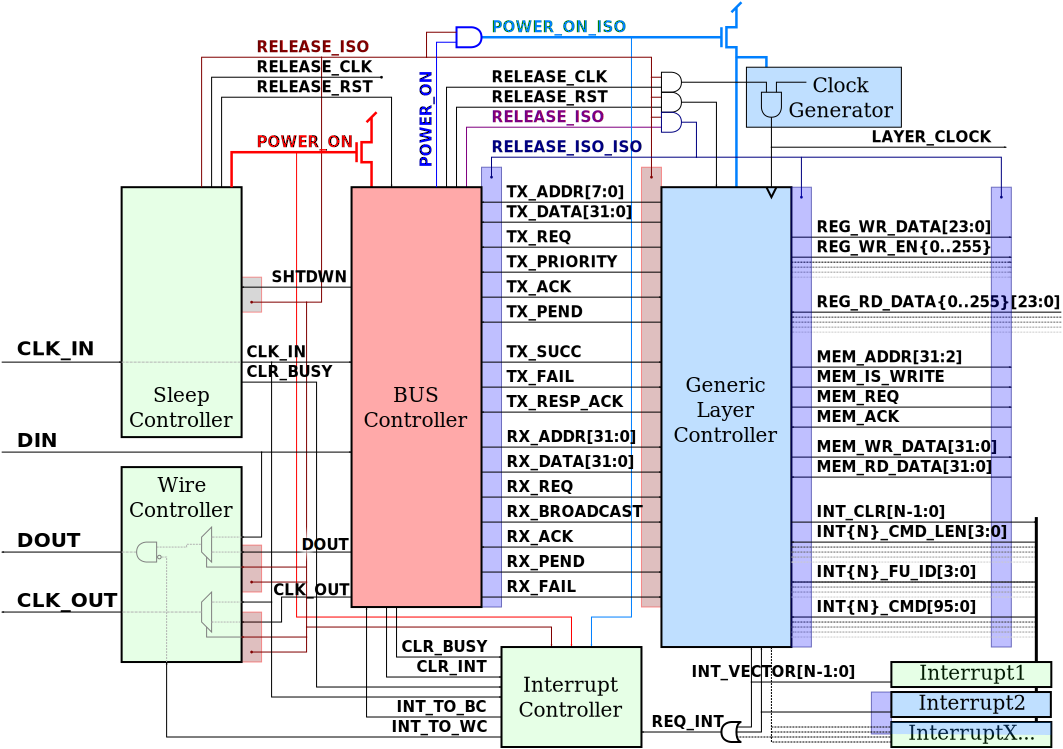
\includegraphics[width=\linewidth]{img/block_diagram}
\caption{{\em Implementation block diagram---~}%
The green blocks are always-on components.
The two power-gated power domains are shown in red
(Bus Controller) and blue (Layer Controller).
Module I/O isolation is indicated by the large rectangles controlled by
{\tt ISO(LATE)} signals.
Circuits elements presented are for conceptual understanding not final design
of glitch-free logic. The global reset signal is omitted for clarity.}
\label{fig:block-diagram}
\end{figure}

The four standard power control signals are:

\begin{quote}
\begin{tabular}{r l l c c}
  Signal Name        & Function  & Power-Up & Power-Down \\
  \hline \hline
  {\tt POWER\_ON}    & Controls Power-Gating           & \nth{1} & \nth{2} \\
  {\tt RELEASE\_CLK} & Supply Clock to Internal Logic  & \nth{2} & \nth{2} \\
  {\tt RELEASE\_ISO} & Electrically Isolate Module I/O & \nth{3} & \nth{1} \\
  {\tt RELEASE\_RST} & (De)Assert Reset                & \nth{4} & \nth{2} \\
\end{tabular}
\end{quote}

The {\tt RELEASE\_CLK} signal may be omitted if the power-gated layer does not
have an internal clock.

\newpage

\subsection{Module Block Details}
This section provides details on the inner workings of each of the supplied
modules.

\subsubsection{Sleep Controller}
The job of the sleep controller is to wake the bus controller
when a message on the bus begins. The sleep controller is also responsible for
powering down the bus controller when requested, using edges from \bus to do
so. For layers capable of waking on events other than \bus transactions, the
sleep controller may be extended or need to coordinate with other sleep
controllers. This document assumes only a basic sleep controller.

\paragraph{Signals}

\subparagraph{Power Signals}
The sleep controller uses both edges of the {\tt CLK\_IN} signal to generate
the power signals. The rising edge that resolves arbitration is used to
release the power gating. The falling edge (Priority~Drive) is unused and
reserved for implementations that require a {\tt RELEASE\_CLK} signal. The
next rising edge (Priority~Latch) drives {\tt RELEASE\_RST} and the falling
edge (Begin~Transmission) drives {\tt RELEASE\_ISO}. The next rising edge
latches Bit~0 of the transmission.

\subparagraph{\bus Signals}
The sleep controller samples and passes through the \bus~{\tt CLK\_IN} signal.
The sleep controller uses this line to clock its internal state machine.
The sleep controller and the bus controller can be safely considered
synchronous modules with respect to one another as they both rely on the \bus 
{\tt CLK\_IN} signal to provide a clock.

\subparagraph{Module Signals}
The sleep controller has only one non-reset input signal: {\tt SHTDWN}. This
signal is asserted by the bus controller to request that it be put to sleep.
This signal is sampled synchronously with the \bus clock. The {\tt SHTDWN}
signal may only be asserted during the falling edge Drive~Control~Bit~1.

The sleep controller is also responsible for generating a {\tt CLR\_BUSY}
output signal when it powers off the bus controller. This signal is normally
generated by the bus controller at the end of \bus transactions and is used to
indicated to the interrupt controller that the bus is no longer busy.

\subsubsection{Wire Controller}
The wire controller is responsible for physically driving the \bus wires. This
separation is necessary to ensure that the data and clock lines are forwarded
even when the bus controller is power gated.
The wire controller is very simple module, conceptually it is little more than
a mux that either forwards the values coming in from the bus or values coming
from the bus controller. The wire controller also must allow for the interrupt
controller to induce a glitch on the bus for wakeup as discussed in the Power
Design section of the {\em \bus Specification}.

Changing the wire controller muxes requires extreme care to ensure that
glitches are not introduced. In practice, this means only changing the clock
mux signal when {\tt CLK\_IN} is already high. The data mux is more
complicated. During Idle, the data line is high, any glitches while pulling it
low (so long as it ultimately is held low) will be significantly shorter than
$t_{long}$ and therefore ignored. During transmission, the state of the data
line is not always known when control transitions are required. \bus ignores
the data line while the clock is low. Any potentially glitch-inducing changes
to the data mux must occur on the falling edge of clock to avoid uncertainty.

The wire controller also facilitates external interrupts as a wakeup source
via a {\em glitch inducer}. The goal of the glitch inducer circuit is to
request a bus arbitration cycle and {\em lose} it. Nominally, this results in
no winner of arbitration and the bus will quickly reset. However, the glitch
inducer logic must also correctly handle the case where another node was
performing genuine arbitration at the same time and a real message takes
place.

\subsubsection{Interrupt Controller}
The interrupt controller is responsible for directing interrupt events to the
appropriate modules at the appropriate times. The destination of an interrupt
event depends on the current power state of the bus controller and layer
controller.

If the layer controller is powered on, the interrupt controller blocks the
interrupt signal as the layer controller will handle the interrupt and
generate any appropriate messages. If the layer controller is powered off,
however, the bus controller must wake the layer controller. To do this, the
bus controller must harvest edges from \bus. To generate the power signals,
the bus controller must observe a transaction while the {\tt INT\_TO\_BC}
signal is asserted. To generate these edges, the interrupt controller must
induce a glitch.

\subparagraph{A Subtle Detail:}
Extreme care must be taken when this glitch is induced, in particular it is
important to ensure that \bus is idle so that a real glitch is not created.
The simple approach would be to ask the bus controller to simply export a
``bus~busy'' signal, asserted while a transmission is active. Such a signal
is not sufficient, however. If a bus controller is not powered on, it is
incapable of asserting busy. If two nodes have interrupts near each other in
time, the first node will induce a glitch unobserved by the second node. If
an interrupt occurs on the second node between end of $t_{long}$ and resultant
falling edge of {\tt CLK\_IN} and the rising edge for arbitration, the second
node will unintentionally and worse unknowingly win arbitration. As the node
does not know that it has won arbitration, it will never end the transmission
and the \bus will be locked until the master node's watchdog counter expires.

To avert this issue, the interrupt controller keeps an internal sense of
``bus~busy''.  The interrupt controller latches the bus as busy whenever {\tt
CLK\_IN} goes low. The internal busy signal is then cleared by an explicit
signal from the bus controller at the end of \bus transactions. As a special
case, the sleep controller must clear the busy status when it powers the bus
controller down as the bus controller will be powered off at the end of the
transaction and incapable of generating the signal. This clear busy signal is
internally treated as the last step in the power-down sequence.

\subsubsection{Bus Controller}
The bus controller is responsible for
handling all possible bus events, including generating acknowledgments if it
is the target of a transaction. The bus controller is only obligated to hold
one word of a transaction, devices wishing to receive messages longer than one
word in length must have a local FIFO to store partial messages in their layer
controller.

\paragraph{Signals}

\subparagraph{Power Signals}
The bus controller provides the same power control signals to the layer
controller that the sleep controller provided to the bus controller. For basic
layers, the bus controller is responsible for waking and sleeping the layer
controller.

The bus controller should only wake the layer controller if there is a message
of {\em non-zero} length being transmitted to the layer's address. In practice
this means the bus controller should not begin waking the layer controller
until it has received the {\em third} data bit. Layer controllers should {\bf
not} be awoken for broadcast messages.

Once the bus controller elects to begin waking the layer controller, it {\bf
must} wake the layer controller completely. Even if another data bit is never
sent (Interrupt) after the bus controller elects to wake the layer controller,
the bus controller still has the Begin~Interrupt, Control~Bit~0,
Control~Bit~1, and Begin~Idle edges to use to wake the layer controller.

The bus controller will indicate an erroneous wake-up by asserting {\tt
RX\_FAIL} signal. The layer controller must acknowledge ({\tt RX\_ACK}) the
erroneous transmission before the bus controller is capable of receiving
another message. This enables the layer controller to take action to put
itself back to sleep after a spurious wakeup.

\subparagraph{\bus Signals}
While the bus controller is not directly connected to the external pads for
all \bus signals, it does use all \bus inputs:

\begin{quote}
\begin{tabular}{r l l}
  {\sc  input} & {\tt CLK\_IN} & Bus Clock In \\
  {\sc output} & {\tt CLK\_OUT} & Bus Clock Out \\
  {\sc  input} & {\tt DIN} & Bus Data In \\
  {\sc output} & {\tt DOUT} & Bus Data Out \\
\end{tabular}
\end{quote}

\subparagraph{Module Signals}
\label{sec:bus-controller-signals-module}
~

\begin{quote}
\begin{tabular}{r l l}
  {\sc  input} & {\tt RESET} & Global system reset \\
  {\sc output} & {\tt SHTDWN} & Request power gating \\
  & & \\
  {\sc  input} & {\tt TX\_ADDR[7:0]} & Address to transmit \\
  {\sc  input} & {\tt TX\_DATA[31:0]} & Data to transmit \\
  {\sc  input} & {\tt TX\_REQ} & Request to transmit \\
  {\sc  input} & {\tt TX\_PRIORITY} & Is high priority message? \\
  {\sc output} & {\tt TX\_ACK} & Acknowledge request to transmit \\
  {\sc  input} & {\tt TX\_PEND} & More data pending \\
  & & \\
  {\sc output} & {\tt TX\_SUCC} & Transmit successful \\
  {\sc output} & {\tt TX\_FAIL} & Transmit failed \\
  {\sc  input} & {\tt TX\_RESP\_ACK} & Acknowledge TX successful / fail \\
  & & \\
  {\sc output} & {\tt RX\_ADDR[31:0]} & Destination address of RX'd packet \\
  {\sc output} & {\tt RX\_DATA[31:0]} & Data received \\
  {\sc output} & {\tt RX\_REQ} & Data is ready \\
  {\sc output} & {\tt RX\_BROADCAST} & RX'd message was a broadcast message \\
  {\sc  input} & {\tt RX\_ACK} & {\tt RX\_DATA} has been saved \\
  {\sc output} & {\tt RX\_PEND} & More data is coming \\
  {\sc output} & {\tt RX\_FAIL} & Abort current RX \\
\end{tabular}
\end{quote}

The bus controller provides a single-word interface to \bus to higher level
modules. To ensure that the bus controller can send a timely ACK for a
received message, modules are obligated to be able to (eventually) receive a
minimum of one word. That is, if the {\tt RX\_REQ} line is raised, the module
{\em must} eventually receive that word by signaling {\tt RX\_ACK}. If another
message is received while {\tt RX\_REQ} is still high, the bus controller will
Interrupt the bus indicating {\tt "01"} ($\sim$EoM, TX/RX Error). This serves
to (i) save bus bandwidth by canceling a message that will not be received,
and (ii) indicate to the transmitting layer that there is still a pending
message (or message part) in the receiving layer.

If the {\tt TX\_PEND} signal is asserted but a {\tt TX\_REQ} for a new word is
not sent by the time the first word has been sent, the bus controller will
Interrupt the bus indicating {\tt "01"} ($\sim$EoM, TX/RX Error). The bus
controller will also assert {\tt TX\_FAIL}, at which point the transaction
must be aborted.

The {\tt RX\_PEND} signal requires special attention. When the {\tt RX\_REQ}
signal rises, if {\tt RX\_PEND} is also high, it indicates that there is more
data to follow. If a module asserts {\tt RX\_ACK} in response it is obligating
itself to receive at least one more word after the current word\footnote{
  This is logically a continuation of the original contract. In an idle state, a
  module has received zero words thus far and is obligated to be able to receive
  one more. If a module ACKs a word while {\tt RX\_PEND} is high, it is
  accepting the current word {\em and} committing to receive the next pending
  word.}.
If a module cannot receive another word beyond the word it is currently
latching, it should ignore {\tt RX\_REQ}.  When the next word is received by
the bus controller, it will detect that {\tt RX\_REQ} is still high and abort
the entire transaction, Interrupting to indicate RX Error. In practice this
means a transmitting node may believe it has sent one more word than was
actually received. As the entire transaction is NAK'd however, the only
implications are for the software flow control estimation, which can
compensate.

For simple nodes that only support single word transactions, this {\tt
RX\_PEND} subtlety is important. Such a node should wire its final
acknowledgment output signal in a manner such as
\begin{quote}
  {\tt TX\_ACK\_out = (RX\_PEND\_in) ? 1'b0 : internal\_ack\_signal;}
\end{quote}
to ensure it does not attempt receipt of multi-word transactions. The {\tt
TX\_PEND} signal can simply be tied low.

\newpage
\paragraph{Parameters}
The bus controller requires relatively little configuration. The only
available parameter is the address(es) that this bus instance should respond
to:

\begin{quote}
\begin{tabular}{l l}
  {\tt ADDRESS}       & Address(es) to receive and acknowledge \\
  {\tt ADDRESS\_MASK} & Which bits of {\tt ADDRESS} are significant \\
\end{tabular}
\end{quote}

%%%%%%%%
\begin{comment}
\paragraph{Optional Signals}
For much more advanced devices that may wish to allow for programmatic or
dynamic address matching, the optional {\tt RX\_ADDR\_VALID} and {\tt
RX\_SHOULD\_ACK} signals are provided. The valid signal will be raised when
the address has been received and is available. The should-ack signal will be
sensed on the next \bus {\tt CLK} edge and will override the internal
comparison if it is high. This has two implications: (i) designs wishing for
complete control should instantiate a bus controller instance that will never
match an address, and (ii) the path to generate the should-ack signal should
be very short to ensure the timing constraint is met.
\end{comment}
%%%%%%%%

\subsubsection{Generic Layer Controller}
\label{sec:generic-layer-controller}
The layer controller is responsible for communicating with the bus controller
and facilitating multi-word transactions. It federates access to the
individual components on a \bus member node. The generic layer controller is
designed such that unused modules (e.g. memory access and control) can be
synthesized out if they are unused.

\paragraph{Power Signals}
The generic layer controller can only be woken by the bus controller. Layers
capable of generating an interrupt while M3 is in sleep mode (e.g. an alarm)
must wire into the glitch inducer via the interrupt controller to wake the
layer and the whole M3 system. The generic layer controller does not output
any power signals.

There is no explicit shutdown signal from the layer controller to the bus
controller. Rather, the layer controller issues a broadcast message announcing
to the bus its intention to shut down. The bus controller will recognize the
special broadcast message and shut down the layer controller once it is sent.
The actual shutdown does not begin until the bus controller successfully
transmits the \texttt{EoM} bit at the end of the transaction.

\paragraph{Module Signals (Bus Side)}
All layer controllers have a common set of signals to interface with the bus
controller, as shown in \autoref{fig:block-diagram}. Details of these
signals are presented in the bus controller documentation:
\ref{sec:bus-controller-signals-module}~\nameref{sec:bus-controller-signals-module}.

\paragraph{Module Signals (Interface Side)}
The generic layer controller expects to communicate with two types of
hardware: a register file and a basic memory. One or both of these may be
instantiated.

\subparagraph{Register File:} The register file is for small, simple
configuration, status, or action bits. It presents an 8~bit address space with
24~bit wide data. Writes are pulse-triggered, with a unique write control line
for each of the registers. Data to read must always be valid, with no
indication that data is being read.

Registers may be smaller than 24~bits. Unused bits for writing should be left
disconnected. Unused bits for reading {\bf must} be tied {\bf low}.

\begin{quote}
\begin{tabular}{r l l}
  {\sc output} & {\tt REG\_WR\_EN\{0..255\}} & Register write enable lines \\
  {\sc output} & {\tt REG\_WR\_DATA[23:0]} & Register data \\
  {\sc  input} & {\tt REG\_RD\_DATA\{0..255\}}[23:0] & Wires from registers \\
\end{tabular}
\end{quote}

\subparagraph{Memory:} The memory interface is for larger amounts of data
(images, audio, packets, etc). Memory is a 32~bit address space with 32~bit
data. The memory space does not alias the register file address space.

The memory interface is a simple two-wire handshake that indicates a request
when signals are valid and an acknowledgment when the data has been latched.
Memory must be fast enough that it can support streaming reads / writes at the
line speed of \bus (see \nameref{sec:interdependencies:frequencies} for detail).

\begin{quote}
\begin{tabular}{r l l}
  {\sc output} & {\tt MEM\_ADDR[31:2]} & Memory address \\
  {\sc output} & {\tt MEM\_IS\_WRITE} & Read/Write selection \\
  {\sc output} & {\tt MEM\_REQ} & Request is ready \\
  {\sc  input} & {\tt MEM\_ACK} & Response is ready \\
  {\sc output} & {\tt MEM\_WR\_DATA[31:0]} & Data to write \\
  {\sc  input} & {\tt MEM\_RD\_DATA[31:0]} & Data that was read \\
\end{tabular}
\end{quote}

\paragraph{Module Signals (Interrupt Interface)}
To generate messages internally, the local node interrupts the layer
controller. Interrupt priority is fixed and ranked by the interrupt index.
Interrupts are non-interruptible and are serviced completely before handling
the next or new interrupt. If an interrupt and a message from the bus arrive
at the same time, the interrupt takes priority.

Conceptually, a local interrupt ``fakes'' the receipt of a message from the
bus, thus the data format is the exact same as bus commands. To generate a
memory {\em write} command for example, the interrupt payload is a memory {\em
read} command, because the response to a memory read request is to generate a
memory write. The \texttt{CMD\_LEN} specifies the length in words of the
payload that is valid. A length of zero indicates that no command should be
executed (the \texttt{FU\_ID} and \texttt{CMD} fields are ignored) and can be
cleared immediately -- this is useful for generating wakeup requests with no
immediate command to execute.

\begin{quote}
\begin{tabular}{r l l}
  {\sc  input} & {\tt INT\_VECTOR[N-1:0]} & Interrupt requests \\
  {\sc output} & {\tt INT\_CLR[N-1:0]} & Clear interrupts \\
  {\sc  input} & {\tt INT\{N\}\_CMD\_LEN[1:0]} & Word length of payload \\
  {\sc  input} & {\tt INT\{N\}\_FU\_ID[3:0]} & Command the LC ``receives'' \\
  {\sc  input} & {\tt INT\{N\}\_CMD[95:0]} & Command payload \\
\end{tabular}
\end{quote}

\subsection{Module Interdependencies}
\label{sec:interdependencies}
In addition to the module signals, the following additional requirements must
be considered for the blocks to operate correctly.

\subsubsection{Clock Domains}
The bus controller and layer controller are on separate clock domains. Care
must be taken with the {\tt REQ} and {\tt ACK} two-wire handshake to ensure
that signals are all double-latched. Double latches should not be required for
the other signals are they are only sampled after the {\tt REQ} or {\tt ACK}
line is stable.

The generic layer controller does not perform double-latching with any of the
signals attached to the register file or memory. These blocks are expected to
run on the same clock as the layer controller. Designs that violate this
assumption must make modifications to ensure signal stability.

\subsubsection{Relative Clock Frequencies}
\label{sec:interdependencies:frequencies}
Nominally, the layer controller would only require activity once every 32~\bus
clock cycles. In practice, however, there is a double-latched, bidirectional
handshake between the bus controller and layer controller. At a minimum then,
the layer controller must be at least $\sfrac{1}{8}$ the speed of the bus.

This timing constraint further extends to the memory if longer bus
transactions are going to be supported. The generic layer controller is a
write-through device, it does not buffer memory requests. Consider the memory
latency in cycles $M$ to be defined as the maximum possible number of cycles
between the assertion of {\tt MEM\_REQ} before the {\tt MEM\_ACK} response is
asserted, then the minimum clock speed of the layer controller and memory is
$\frac{6+M}{32}$ of the bus speed.

There is no upper bound on the layer speed relative to the bus.
Layer controller clock speeds are generally configurable.

\clearpage

%%%%%%%%%%%%%%%%%%%%%%%%%%%%%%%%%%%%
\clearpage
\section{Document Revision History}
\label{sec:revisions}

\begin{itemize}

\item Revision 0.4 {\footnotesize(r12314)} -- July 21, 2015
  \subitem Remove dedicated CPU layer controller
  \subitem Enhance generic layer controller interrupt interface
  \subitem Move messages and register defintions to MPQ in MBus Specification

\item Revision 0.3 {\footnotesize(r7649)} -- Apr 18, 2013
\subitem Add functional unit addresses
\subitem Change addressing to reflect new prefix-style addressing
\subitem Update power-gating details
\subitem Add Wire Controller
\subitem Add Interrupt Controller
\subitem Add Channel~3 Information
\subitem Update layer controller information to match actual design
\subitem Use the word {\em Reserved} in the programmer model

\item Revision 0.2 {\footnotesize(r3194)} -- Mar 4, 2013
\subitem Add power-gating information
\subitem Add {\tt RX\_FAIL} signal
\subitem Solidify Interrupt TODO
\subitem Add {\tt PRIORITY} signal

\item Revision 0.1 {\footnotesize(r2847)} -- Jan 22, 2013
\subitem Initial revision

\end{itemize}


\end{document}
